\section{Sterowanie jednostkami (Zofia Sosińska)}\label{chap:mb}
Gry z możliwością tworzenia drużyny muszą rozwiązć problem zachowania podwładnych. Program może udostępniać
skomplikowaną sztuczną inteligencję dla wojowników, zawsze rozwiązujac konflikt w optymalny sposób, ale w tym przypadku 
użytkownik staje się obserwatorem, a nie dowodzącym, co go znacznie odciąży. Innym podejściem może być zaprojektowanie podwładnych jako 
marionetek bez własnej woli, które będą biernie czekać, aż do otrzymania rozkazu. Wtedy jednak gracz musi skupiać się na 
każdym ruchu zarówno swojej, jak i przeciwnej drużyny tak, aby w porę móc zareagować na wszystkie zmiany, co
jest rozwiązaniem obciążającym dla użytkownika. Przy projektowaniu mechaniki sterowania jednostkami trzeba zachować balans pomiędzy 
dodaniem i odjęciem użytkownikowi zadań, na kórych musi się skupić. Dla każdej gry ta proporcja może być inna, zależnie
od unikalnego charakteru gry.

Przy projektowaniu gry Mount\&Blade studio TaleWorlds Entertainment zdecydowało się zaimplementować mechanikę sterowania jednostkami tak, aby 
dodać do walki element strategii. Gracz bezpośrednio steruje jedynie główną postacią i podczas walki może wydawać rozkazy reszcie. Poprzez
cyfry 0-4 wybiera grupę, do której się odnosi np. łuczników. Po naciśnięciu konkretnego przycisku, po lewej stronie ekranu pojawia się lista dostępnych komend.
Następnie przez klawisze F1-F11 wydaje konkretny rozkaz np. odwrót. Lista znika, sztuczna inteligencja postaci zajmuje się już samym wykonaniem czynności. 
Gracz nie martwi się, czy jednostki znajdą optymalną drogę, 
będą celować w przeciwników, czy z nimi walczyć. Zachowany jest więc przyjemny balans pomiędzy podejmowaniem kluczowych decyzji, a byciem odciążonym przez mechanizmy sztucznej inteligencji.

\begin{figure}[h!tbp]
    \centering
    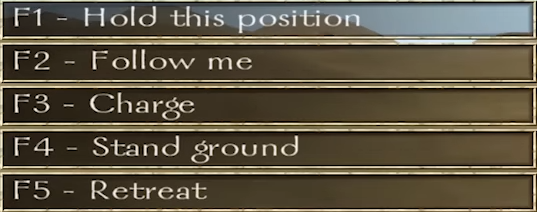
\includegraphics[width=0.9\textwidth]{images/ui/commandsMountBla.png}
    \caption{Wykaz dostępnych rozkazów z gry Mount\&Blade.}\label{fig:MountnBlade}
    \label{fig:mnb}
\end{figure}
